\documentclass{article}
\usepackage[utf8]{inputenc}
\usepackage[brazil]{babel}
\usepackage{tikz}
\usetikzlibrary{arrows.meta, positioning}
\usepackage{amsmath, amssymb, amsfonts}
\usepackage{graphicx}
\usepackage{booktabs}
\usepackage{bm}
\usepackage{hyperref}


\usepackage{pgfplots}
\pgfplotsset{compat=1.17}
\usepackage{caption}
\usepackage{subcaption}
\usepackage{geometry}
\geometry{margin=2cm}



\begin{document}

\title{Sistemas de equações de diferenças}
\date{}


\maketitle


\section*{Enunciado}

Um economista está interessado na variação do preço de um único produto. Observa-se que um preço elevado do produto no mercado atrai mais fornecedores. No entanto, o aumento da quantidade ofertada tende a reduzir o preço. Com o tempo, há uma interação entre preço e oferta. O economista propõe o seguinte modelo, onde $P_n$ representa o preço no ano $n$, e $Q_n$ representa a quantidade:

\[
\begin{aligned}
P_{n+1} &= P_n - 0{,}1(Q_n - 500) \\
Q_{n+1} &= Q_n + 0{,}2(P_n - 100)
\end{aligned}
\]

\begin{enumerate}
  \item[(a)] O modelo faz sentido intuitivamente? Qual o significado das constantes 100 e 500? Explique o significado dos sinais $-0{,}1$ e $0{,}2$.
  \item[(b)] Teste as condições iniciais abaixo e descreva o comportamento de longo prazo:

  \begin{center}
    \begin{tabular}{lcc}
      \toprule
      \textbf{Caso} & \textbf{$P_0$} & \textbf{$Q_0$} \\
      \midrule
      A & 100 & 500 \\
      B & 200 & 500 \\
      C & 100 & 600 \\
      D & 100 & 400 \\
      \bottomrule
    \end{tabular}
  \end{center}

\end{enumerate}

\section*{Resolução}

\subsection*{(a) Interpretação do modelo}

As equações do modelo são:

\[
\begin{aligned}
P_{n+1} &= P_n - 0{,}1(Q_n - 500) \\
Q_{n+1} &= Q_n + 0{,}2(P_n - 100)
\end{aligned}
\]

\paragraph{O modelo faz sentido intuitivamente?}

Sim, o modelo reflete bem a lógica econômica básica de oferta e demanda:

\begin{itemize}
\item Quando o \textbf{preço sobe}, os produtores tendem a ofertar
  mais. Isso aparece na equação de $Q_{n+1}$, onde $Q$ aumenta se
  $P_n > 100$.

  A equação para o preço é:
  \[
    P_{n+1} = P_n - 0{,}1(Q_n - 500)
  \]
  \begin{itemize}
  \item Se $Q_n > 500$, então $P_{n+1} < P_n$: excesso de oferta reduz
    o preço.
  \item Se $Q_n < 500$, então $P_{n+1} > P_n$: escassez aumenta o
    preço.
  \item Portanto, $Q = 500$ é a quantidade que mantém o preço estável.
  \end{itemize}

  
\item Quando a \textbf{oferta aumenta}, o excesso de produto no mercado
  tende a reduzir o preço. Isso aparece na equação de $P_{n+1}$, onde
  $P$ diminui se $Q_n > 500$.

  A equação para a quantidade é:
  \[
    Q_{n+1} = Q_n + 0{,}2(P_n - 100)
  \]
  \begin{itemize}
  \item Se $P_n > 100$, então $Q_{n+1} > Q_n$: preço alto incentiva
    maior oferta.
  \item Se $P_n < 100$, então $Q_{n+1} < Q_n$: preço baixo desincentiva
    a oferta.
  \item Portanto, $P = 100$ é o preço que mantém a quantidade estável.
\end{itemize}
\end{itemize}

\paragraph{Significado das constantes 100 e 500}

\begin{itemize}
\item $100$: é o \textbf{preço de equilíbrio} — quando $P_n = 100$, a
  oferta não muda ($Q_{n+1} = Q_n$).
\item $500$: é a \textbf{quantidade de equilíbrio} — quando
  $Q_n = 500$, o preço não muda ($P_{n+1} = P_n$).
\end{itemize}

\paragraph{Significado dos sinais $-0{,}1$ e $+0{,}2$}

\begin{itemize}
\item $-0{,}1$: indica que há uma \textbf{reação negativa do preço} ao
  excesso de oferta (preço cai se $Q_n > 500$).
\item $+0{,}2$: indica que há uma \textbf{reação positiva da oferta} ao
  aumento de preço (quantidade aumenta se $P_n > 100$).
\end{itemize}

\subsection*{(b) Análise dos Casos}

\paragraph{Ponto de equilíbrio (fixo):} resolver o sistema
\[
  \begin{cases}
    P_{n+1} = P_n \Rightarrow Q_n = 500\\
    Q_{n+1} = Q_n \Rightarrow P_n = 100
  \end{cases}
\]
\[
  \Rightarrow (P^*, Q^*) = (100, 500)
\]


\paragraph{Caso A: $P_0 = 100$, $Q_0 = 500$}

\[
\begin{aligned}
P_1 &= 100 - 0{,}1(500 - 500) = 100 \\
Q_1 &= 500 + 0{,}2(100 - 100) = 500
\end{aligned}
\]

\textit{Esse par é um ponto fixo: o sistema permanece nele indefinidamente.}

\textbf{Conclusão:} Equilíbrio estável.

\paragraph{Caso B: $P_0 = 200$, $Q_0 = 500$}

\[
\begin{aligned}
P_1 &= 200 - 0{,}1(500 - 500) = 200 \\
Q_1 &= 500 + 0{,}2(200 - 100) = 520 \\
P_2 &= 200 - 0{,}1(520 - 500) = 198 \\
Q_2 &= 520 + 0{,}2(200 - 100) = 540 \\
P_3 &= 198 - 0{,}1(540 - 500) = 194 \\
Q_3 &= 540 + 0{,}2(198 - 100) = 559{,}6
\end{aligned}
\]

\textit{O preço começa alto e a quantidade cresce, mas o preço começa a cair, indicando tendência de retorno ao equilíbrio.}

\textbf{Conclusão:} Sistema oscila, mas parece tender ao ponto fixo $(100, 500)$.

\paragraph{Caso C: $P_0 = 100$, $Q_0 = 600$}

\[
\begin{aligned}
P_1 &= 100 - 0{,}1(600 - 500) = 90 \\
Q_1 &= 600 + 0{,}2(100 - 100) = 600 \\
P_2 &= 90 - 0{,}1(600 - 500) = 80 \\
Q_2 &= 600 + 0{,}2(90 - 100) = 598 \\
P_3 &= 80 - 0{,}1(598 - 500) = 70{,}2 \\
Q_3 &= 598 + 0{,}2(80 - 100) = 594
\end{aligned}
\]

\textit{Preço vai caindo, quantidade também começa a cair.}

\textbf{Conclusão:} Sistema retorna lentamente ao equilíbrio.

\paragraph{Caso D: $P_0 = 100$, $Q_0 = 400$}

\[
\begin{aligned}
P_1 &= 100 - 0{,}1(400 - 500) = 110 \\
Q_1 &= 400 + 0{,}2(100 - 100) = 400 \\
P_2 &= 110 - 0{,}1(400 - 500) = 120 \\
Q_2 &= 400 + 0{,}2(110 - 100) = 402 \\
P_3 &= 120 - 0{,}1(402 - 500) = 129{,}8 \\
Q_3 &= 402 + 0{,}2(120 - 100) = 406
\end{aligned}
\]

\textit{Preço e quantidade estão subindo juntos, afastando-se do equilíbrio.}

\textbf{Conclusão:} Pode levar a oscilações crescentes ou retorno lento, dependendo da dinâmica.


\paragraph{Resumo:}

\begin{center}
\begin{tabular}{lccc}
\toprule
\textbf{Caso} & \textbf{Comportamento} & \textbf{Convergência} \\
\midrule
A & Já está no equilíbrio & $(100,500)$ \\
B & $P$ cai, $Q$ sobe & Converge para $(100,500)$ \\
C & $P$ cai, $Q$ cai & Converge para $(100,500)$ \\
D & $P$ sobe, $Q$ sobe & Converge para $(100,500)$ \\
\bottomrule
\end{tabular}
\end{center}



\subsection*{Simulações Numéricas (Gráficos)}

\begin{center}
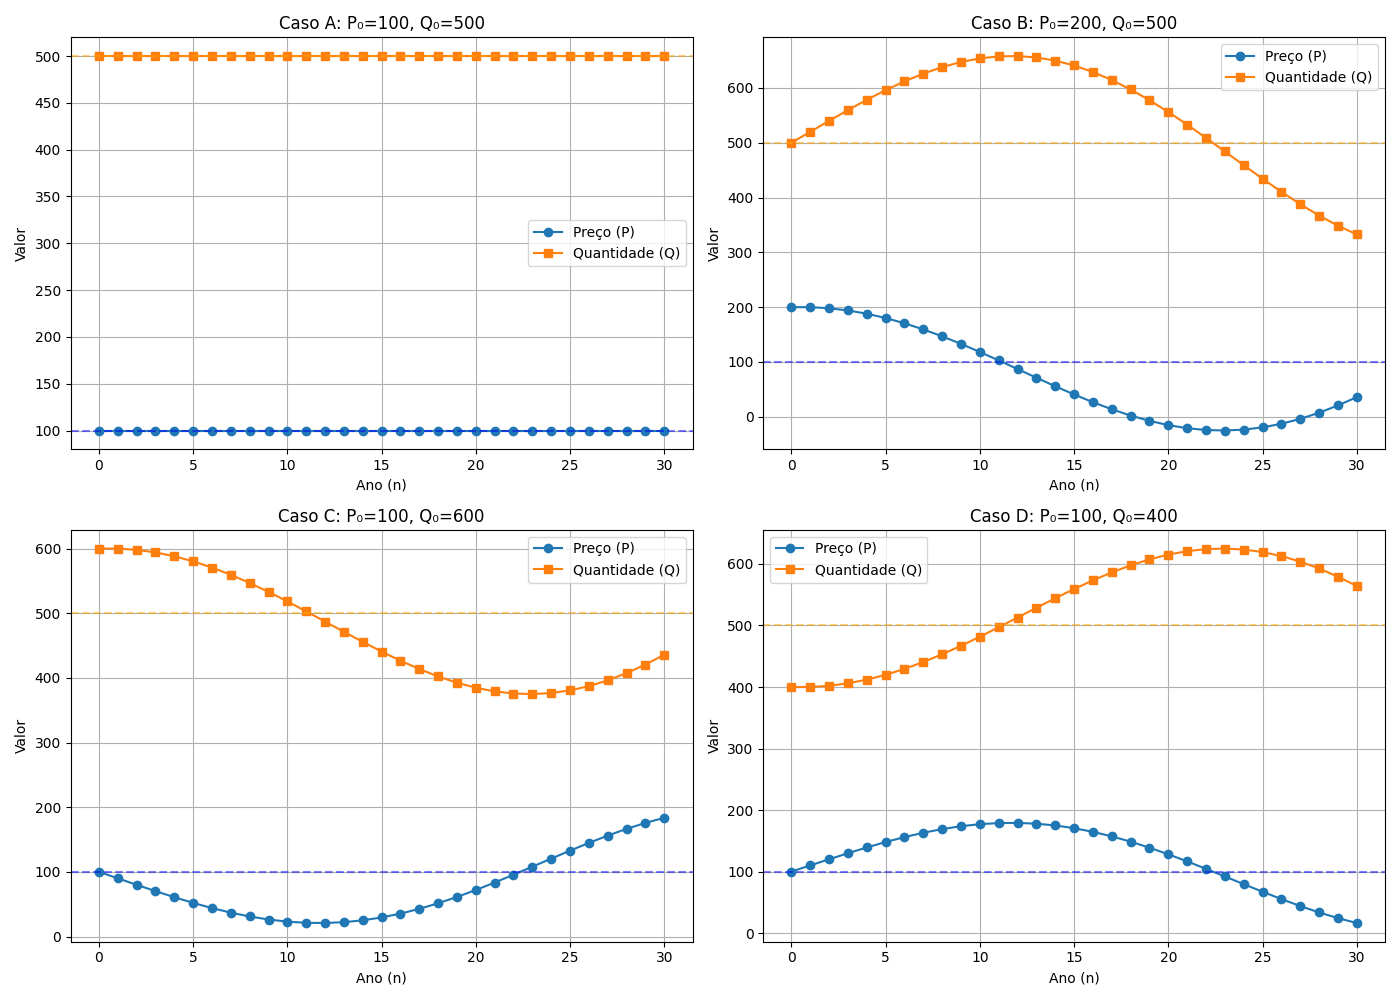
\includegraphics[width=0.9\linewidth]{simulacao.png}
\end{center}

As curvas mostram a convergência de $P$ e $Q$ para o equilíbrio $(100,500)$ em todos os casos testados.

\subsection*{Gráfico de Fase (P vs Q)}

\begin{center}
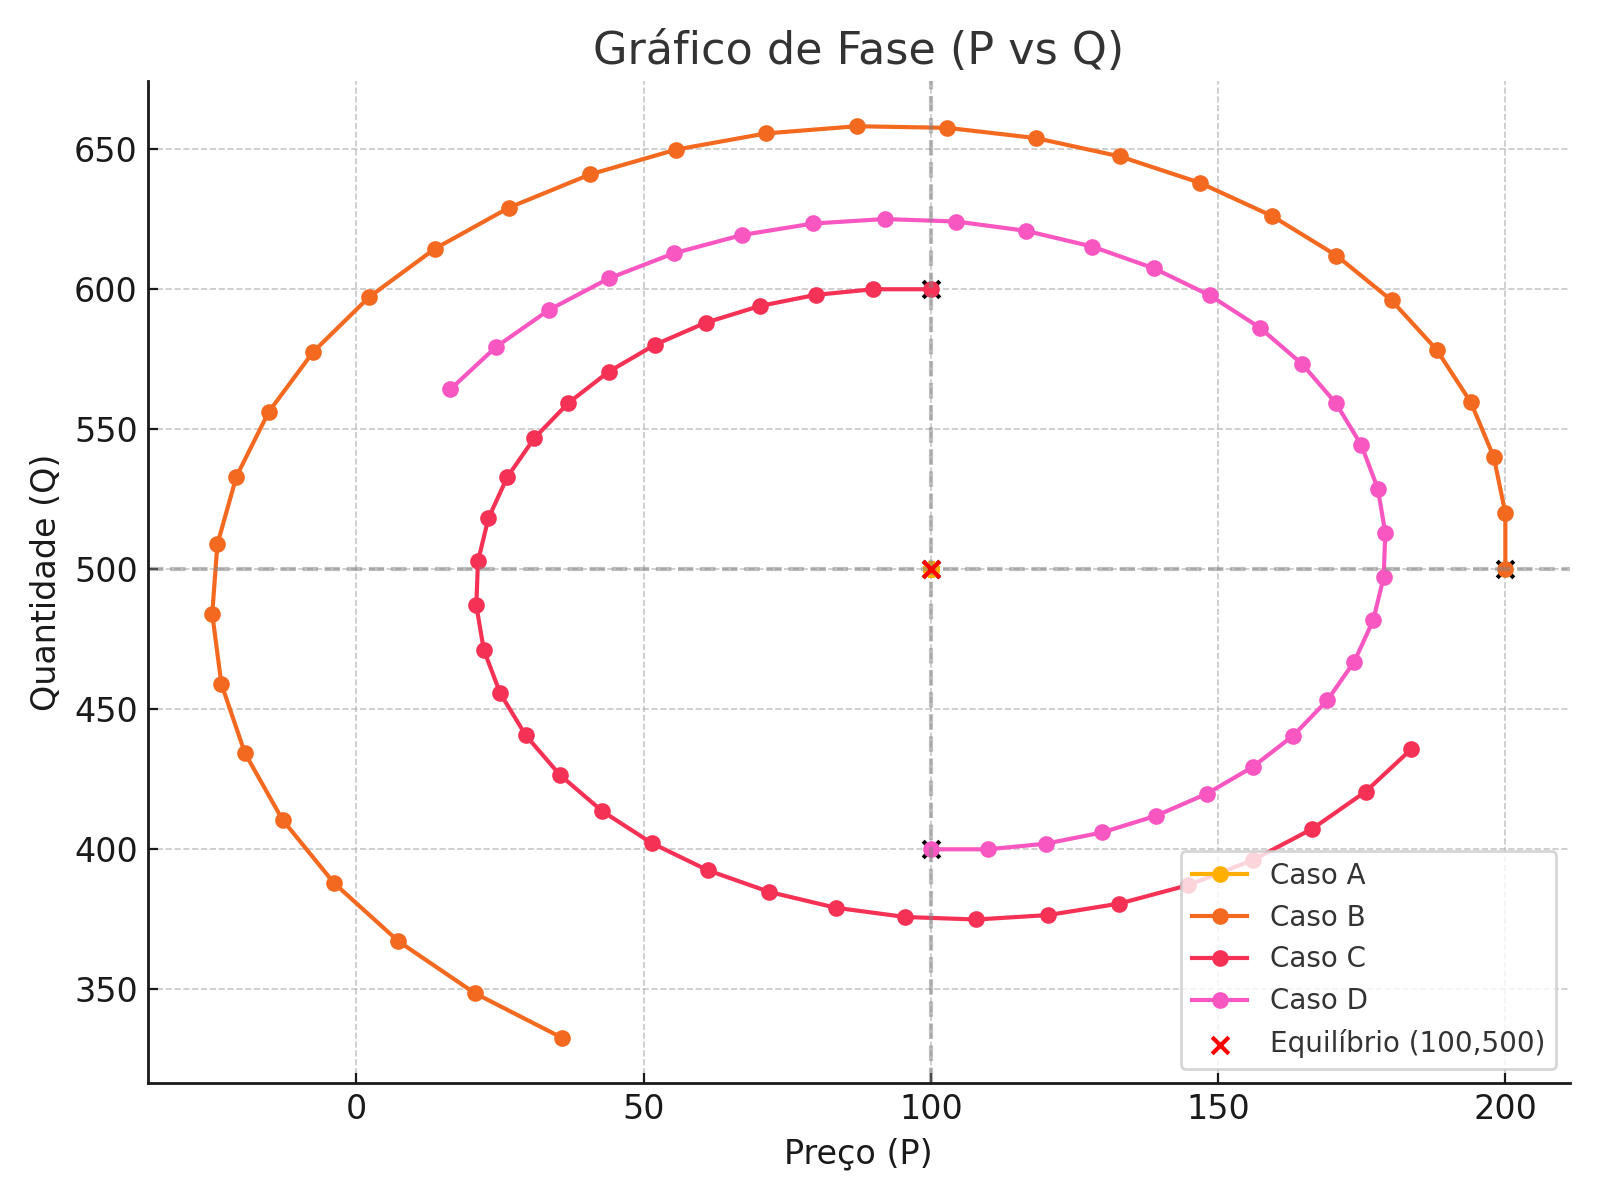
\includegraphics[width=0.7\linewidth]{fase.png}
\end{center}

O gráfico de fase acima mostra a evolução conjunta de preço ($P$) e quantidade ($Q$) para os diferentes casos iniciais.  
As trajetórias convergem para o ponto de equilíbrio $(P^*, Q^*) = (100, 500)$, evidenciando a estabilidade do sistema dinâmico.

O ponto vermelho indica o equilíbrio, e os marcadores "x" são os pontos iniciais de cada trajetória.




\end{document}
\end{document}

